\newpage
\section{Eksamensopgave 6 - Dynamik}
\begin{figure}[h!]
    \centering
    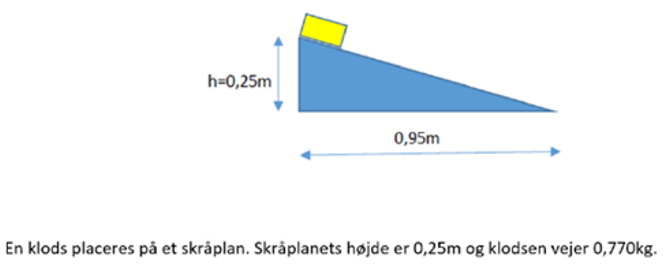
\includegraphics[width=0.8\textwidth]{figures/dynamik.png}
    \caption{Dynamik opgave}
\end{figure}
\subsection{Lav en skitse, der viser hvilke kræfter der virker klodsem og forklar hvilke typer kræfter, der er tale om}
\begin{figure}[h!]
    \centering
    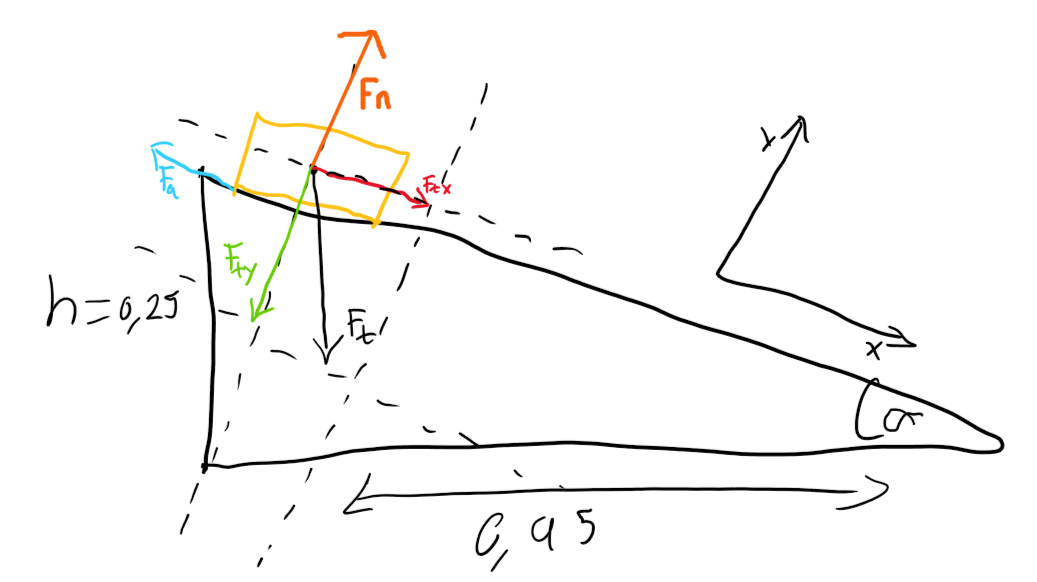
\includegraphics[width=0.6\textwidth]{figures/dynamikskitse.png}
    \caption{Skitse med kræfter}
\end{figure}
\begin{equation*}
    F_{TX} = m \cdot g \cdot cos(\alpha)
\end{equation*}
\begin{equation*}
    F_{TX} = 0,77kg \cdot 9,82\frac{m}{s^{2}} \cdot sin(14,74^{\circ}) = 1,92N
\end{equation*}
\begin{equation*}
    F_{TY} = m \cdot g \cdot sin(\alpha)
\end{equation*}
\begin{equation*}
    F_{TX} = 0,77kg \cdot 9,82\frac{m}{s^{2}} \cdot cos(14,74^{\circ}) = 7,31N
\end{equation*}
Vinklen blev beregnet i opgave 3
\subsection{Bestem tyndekraften på klodsen}
For at bestemme tyngdekræften på klodsen kan vi bruge denne formel.
\begin{equation*}
    F_{t} = m \cdot g
\end{equation*}
Hvor ~$F_{t}$ er tungdekræften, m er massen af vores objekt og g er tyngdeaccelerationen.
\begin{equation*}
    F_{t} = 0,770kg \cdot 9,82\frac{N}{kg} = 7,56N
\end{equation*}
\subsection{Hvor stor skal gnidningskoefficenten mellem skråplan og kolds mindst være, for at klodsen ikke bevæger sig?}
For at beregne opgaven skal vi vide hældningen på den plan klodsen er på. Hældningen kan vi beregne med tangens.
\begin{equation*}
    tan(v)=\frac{Mod}{Hos}
\end{equation*}
\begin{equation*}
    tan(v)=\frac{0,25m}{0,95m}
\end{equation*}
Nu skal $v$ isoleres ved at tage $tan^{-1}$ på begge sider og får så derfor.
\begin{equation*}
    \mathcolorbox{yellow}{v=tan^{-1}(\frac{0,25m}{0,95m}) = 14,74^{\circ}}
\end{equation*}

Nu når vi har vinklen skal vi bruge formlen for gnidningskraften som ser sådan ud.
\begin{equation*}
    m \cdot g \cdot sin(\alpha) = m \cdot g \cdot cos(\alpha) \cdot \mu
\end{equation*}
m = masse\newline
g = tyngdeaccelerationen\newline
$\alpha$ = vinkel\newline
$\mu$ = gnidningskoefficenten\newline\newline

Nu skal vi have isoleret my [$\mu$]. Det første man opdager er at $m \cdot g$ står på begge sider af lighedstegnet og derfår går de ud med hinanden og bliver til.
\begin{equation*}
    sin(\alpha) = cos(\alpha) \cdot \mu
\end{equation*}
Nu for at få $\mu$ til at stå alene skal vi dividere med $cos(\alpha)$ på begge sider, og bliver derfor til.
\begin{equation*}
    \mathcolorbox{yellow}{\frac{sin(\alpha)}{cos(\alpha)} = \mu}
\end{equation*}
Og der er så vores formel for at bestemme den mindste værdi gnidningskoefficenten skal være for at vores objekt vil bevæge sig.\newline
Nu skal vi bare indtaste vores værdier ind i formlen for at finde gnidningskoefficenten.
\begin{equation*}
    \mathcolorbox{yellow}{\mu = \frac{sin(14,74^{\circ})}{cos(14,74^{\circ})} = 0,26}
\end{equation*}